% https://tex.stackexchange.com/a/337218
\documentclass{beamer}
\usepackage{tikz}
\usetikzlibrary{arrows,positioning,trees} 

\tikzset{
    >=stealth',
    punkt/.style={
        circle,
        draw, 
        fill=blue!30,
        text centered},
    level 1/.style={sibling angle=120, level distance=1cm},
    edge from parent/.style= {draw=none},
}

\begin{document}
\begin{frame}
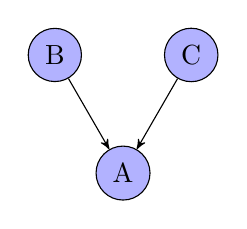
\begin{tikzpicture}

\coordinate (main) at (0,0) [clockwise from=270]
    child { node[punkt] (1) {A}}
    child { node[punkt] (2) {B}}
    child { node[punkt] (3) {C}}
;

\draw[->] (2) -- (1);
\draw[->] (3) -- (1);

\end{tikzpicture}
\end{frame}
\end{document}
